\documentclass[12pt, a4paper]{article}

% Ru lang stuff
\usepackage [utf8x] {inputenc}
\usepackage [T2A] {fontenc}

% running titles 
\usepackage{fancybox}
\usepackage{fancyhdr}

% for last page number
\usepackage{lastpage}

%for colored tablets cells
\usepackage{colortbl}

% for Ru text in formulas
\usepackage[warn]{mathtext}

% for captions 
\usepackage[labelsep=period]{caption}
\usepackage{capt-of}

% for colored hyperrefs
\usepackage{xcolor}
\usepackage{hyperref}

% for pictures 
\usepackage{graphicx}

% for coll math
\usepackage{amsmath}

% path to all pictures
\graphicspath{{picks/}}

% for enumerates
\usepackage[shortlabels]{enumitem}

% for diff running titles on pages with diff parity
\usepackage{ifthen}
\usepackage{pdfpages}
\usepackage[strict]{changepage}

%for drawings
\usepackage{tikz}
\usetikzlibrary{calc}
\usetikzlibrary{decorations.pathmorphing}

% for good text in tablets
\usepackage{array}

% upgrading tables
\newcolumntype{P}[1]{>{\centering\arraybackslash}p{#1}}
\newcolumntype{M}[1]{>{\centering\arraybackslash}m{#1}}


% dock fields 20 15 15 35
\usepackage[left=12mm, top=12mm, right=15mm, bottom=28mm, nohead, footskip=10mm]{geometry}

% for cool tables
\usepackage{multirow}

% for different section/subsection/subsubsection styles in contents and doc
\usepackage[english, russian]{babel}

\usepackage{amsmath}

% for cool tables
\usepackage{tabularx}

\newcommand{\sect}[2] {
    \addtocounter{section}{1}
    \section*{\Huge\thesection.\,#1}
    \addcontentsline{toc}{subsection}{ \texorpdfstring{\thesection.\qquad\qquad #2}{Lg}}
}

\newcommand{\subsec}[2] {
    \addtocounter{subsection}{1}
    \subsection*{\thesubsection.\,#1}
    \addcontentsline{toc}{subsection}{ \texorpdfstring{\quad \thesubsection.\qquad\ #2}{Lg}}
}

\newcommand{\subsubsec}[2] {
    \addtocounter{subsubsection}{1}
    \subsubsection*{\thesubsubsection.\,#1}
    \addcontentsline{toc}{subsection}{ \texorpdfstring{\quad\quad\ \thesubsubsection. #2}{Lg}}
}
%-------------------------------------------------------------------------%

% for easy mini pages with shifts
\newcommand{\shiftedText}[3]{
\hspace*{#1}\begin{minipage}[t]{#2}
#3
\end{minipage}
}

\newcolumntype{P}[1]{>{\centering\arraybackslash}p{#1}}

% page style setup (for running titles)
\fancypagestyle{plain}{ %
\fancyhf{} % remove everything

 % lines parameters
\renewcommand{\headrulewidth}{0pt}
\renewcommand{\footrulewidth}{0pt}

% running titles contents
\fancyfoot[L]{\ifthenelse{\isodd{\thepage}}{Работа 1.1.4}{\thepage}}
\fancyfoot[R]{\ifthenelse{\isodd{\thepage}}{\thepage}{Работа 1.1.4}}
}

% choosing page style with our running titles
\pagestyle{plain}

\tolerance = 10000

\title{Лабораторная работа №1.1.4}
\author{Mikhail Pavlov \thanks{MIPT}}
\date{September, 2021}
\begin{document}


\shiftedText{0.5cm}{14cm}
{
    \begin{center}
    \vspace*{1.0cm}    
        
        {\bf\Huge Работа 1.1.4 }
        
    \vspace*{0.2cm}    
        
        {\bf\LARGE Измерение интенсивности радиационного фона }
        
    \vspace*{0.8cm}
        {\LARGE Работу выполнил Павлов Михаил Б01-109 }
        
    \vspace*{1.6cm}
    
    \end{center}
    
    {\bf\noindent Цель работы: }  применение методов обработки экспериментов для изучения статистических закономерностей при измерении интенсивности радиационного фона.

    \vspace*{0.6cm}
    
    {\bf\noindent В работе используются: } счётчик Гейгера-Мюллера (СГС-6), блок питания, компьютер с интерфейсом связи со счётчиком.

}

\fancypagestyle{plain}{ %
\fancyhf{} % remove everything

 % lines parameters
\renewcommand{\headrulewidth}{0pt}
\renewcommand{\footrulewidth}{0pt}
% running titles contents
\fancyfoot[L]{\ifthenelse{\isodd{\thepage}}{Работа 1.1.4}{\thepage}}
\fancyfoot[R]{\ifthenelse{\isodd{\thepage}}{\thepage}{Работа 1.1.4}}
}

% choosing page style with our running titles
\pagestyle{plain}

\tolerance = 10000

\vspace*{0.6cm}

        {\Large 1. Аннотация \\}
        Поток космических частиц, которые составляют значительную часть радиационного фона, изменяется со временем случайным образом.
        Если изменения происходят около какого-либо значения, говорят, что величина флуктуирует. 
        Тогда её характеристики - среднее значение и среднеквадратичное отклонение от него. 
        Их интенсивность можно оценить по ионизации, которую они производят. 
        Для этого используется специальный прибор счётчик Гейгера-Мюллера.
        Счётчик представляет собой наполненный газом сосуд с двумя электродами.
        Один электрод - металлический цилиндр, другой - тонкая нить, натянутая вдоль цилиндра.
        Для работы необходимо напряжение в 400В. Частицы космических лучей ионизируют газ, которым наполнен счётчик, а также выбивают электроны из его стенок.

        \noindent\begin{minipage}[c]{0.67\textwidth}
            \hspace{1cm}Они ускоряются и выбивают новые. Образуется целая лавина электронов, и через счётчик резко увеличивается ток.
            В исходном состоянии электроды и конденсатор заряжены до 400В. Разделительный $C_2$ не пропускает постоянное напряжение источника питания в компьютер.
            При возникновении тока через счётчик заряд на СГС-6 и конденсаторе $C_1$ обеспечивают развитие электронной лавины.
            Если случайные события однородны во времени и каждое последующее событие не зависит от того, когда и как случались предыдущие события, то такой процесс называется пуассоновским и подчиняется Пуассоновскому распределению
            В таком случае средняя квадратичная ошибка равно $\sqrt{\overline{n} }$. \\
            $\overline{n} = \frac{1}{n} \sum_{i = 1}^{N}{n_i}, \sigma = \sqrt{\frac{1}{N} * \sum_{i = 1}^{N}{(n_i - \overline{n})}^2}$. 
            Величина $\overline{n}$ не вполне совпадает с истинным значением. Стандартная ошибка её отклонения
            $\sigma_{\overline{n}} = \frac{\sigma}{\sqrt{N}}. \epsilon_{\overline{n}} = \frac{1}{\sqrt{N} * \overline{n}}$
        \end{minipage}
        \begin{minipage}[c]{0.32\textwidth}
            \begin{center}
                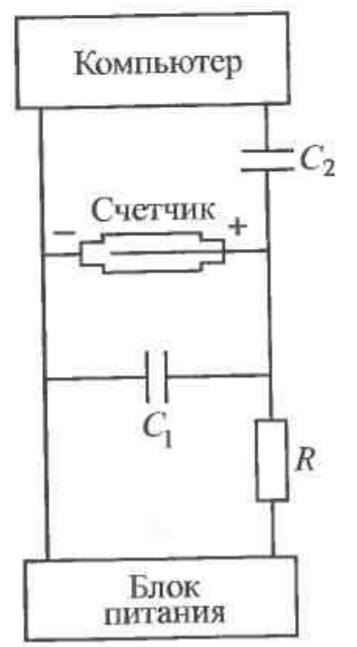
\includegraphics[scale=0.6]{Pics/scheme.jpg} \\
                \textit{\textcolor[HTML]{000000}{Рис. 1. Схема включения \\ счётчика}}
            \end{center}
        \end{minipage}

        \newpage

        {\Large 2. Проведение демонстрационного эксперимента \\}
        Убедимся в том, что 
        \begin{itemize}
            \item измеряемая величина флуктуирует
            \item флуктуации уменьшаются и среднее значение выходит на постоянную величину
            \item флуктуации величины погрешности отдельного измерения уменьшаются
            \item флуктуации величины погрешности среднего значения уменьшаются, а сама величина убывает
          \end{itemize}

          {\Large 3. Результаты измерений и обработка данных \\}
          
          {\large 3.1 Измерение плотности потока космического излучения за 10с. \\}
          \begin{center}
            \begin{tabular}{ |c|c|c|c|c|c|c|c|c|c|c| } \hline
                № опыта & 1 & 2 & 3 & 4 & 5 & 6 & 7 & 8 & 9 & 10 \\ \hline
                0 & 33 & 26 & 32 & 26 & 22 & 31 & 29 & 24 & 33 & 27 \\ \hline
                10 & 27 & 26 & 26 & 20 & 26 & 27 & 22 & 32 & 21 & 36 \\ \hline
                20 & 20 & 26 & 29 & 32 & 26 & 30 & 32 & 27 & 28 & 19 \\ \hline
                30 & 24 & 22 & 21 & 25 & 30 & 29 & 25 & 32 & 38 & 32 \\ \hline
                40 & 29 & 33 & 23 & 31 & 26 & 33 & 27 & 29 & 27 & 27 \\ \hline
                50 & 34 & 25 & 37 & 29 & 29 & 24 & 33 & 21 & 20 & 29 \\ \hline
                60 & 21 & 34 & 37 & 35 & 21 & 31 & 26 & 23 & 32 & 38 \\ \hline
                70 & 34 & 37 & 15 & 29 & 27 & 20 & 24 & 29 & 31 & 26 \\ \hline
                80 & 27 & 23 & 34 & 31 & 15 & 25 & 29 & 36 & 31 & 31 \\ \hline
                90 & 22 & 35 & 29 & 38 & 35 & 24 & 34 & 28 & 19 & 30 \\ \hline
                100 & 34 & 30 & 20 & 27 & 26 & 21 & 25 & 23 & 23 & 18 \\ \hline
                110 & 23 & 27 & 31 & 15 & 38 & 32 & 30 & 17 & 28 & 27 \\ \hline
                120 & 19 & 27 & 23 & 36 & 24 & 18 & 29 & 24 & 28 & 33 \\ \hline
                130 & 35 & 22 & 37 & 37 & 21 & 26 & 35 & 23 & 28 & 34 \\ \hline
                140 & 28 & 34 & 26 & 26 & 35 & 31 & 31 & 38 & 30 & 23 \\ \hline
                150 & 30 & 34 & 29 & 19 & 19 & 23 & 27 & 23 & 30 & 41 \\ \hline
                160 & 27 & 27 & 33 & 17 & 21 & 32 & 27 & 19 & 33 & 25 \\ \hline
                170 & 27 & 26 & 29 & 25 & 26 & 30 & 32 & 22 & 28 & 31 \\ \hline
                180 & 30 & 27 & 29 & 15 & 24 & 27 & 23 & 26 & 20 & 34 \\ \hline
                190 & 30 & 29 & 24 & 27 & 29 & 31 & 25 & 33 & 29 & 34 \\ \hline
            \end{tabular}
            \captionof{table}{Число срабатываний счётчика за 20с.}
            \end{center} 
            
            \begin{center}
                \begin{tabular}{ |c|c|c|c|c|c|c|c|c|c|c| } \hline
                    № опыта & 1 & 2 & 3 & 4 & 5 & 6 & 7 & 8 & 9 & 10 \\ \hline
                    0 & 59 & 58 & 53 & 53 & 60 & 53 & 46 & 53 & 54 & 57 \\ \hline
                    10 & 46 & 61 & 56 & 59 & 47 & 46 & 46 & 59 & 57 & 70 \\ \hline
                    20 & 62 & 54 & 59 & 56 & 54 & 59 & 66 & 53 & 54 & 49 \\ \hline
                    30 & 55 & 72 & 52 & 49 & 70 & 71 & 44 & 47 & 53 & 57 \\ \hline
                    40 & 50 & 65 & 40 & 65 & 62 & 57 & 67 & 59 & 62 & 49 \\ \hline
                    50 & 64 & 47 & 47 & 48 & 41 & 50 & 46 & 70 & 47 & 55 \\ \hline
                    60 & 46 & 59 & 42 & 53 & 61 & 57 & 74 & 47 & 58 & 62 \\ \hline
                    70 & 62 & 52 & 66 & 69 & 53 & 64 & 48 & 42 & 50 & 71 \\ \hline
                    80 & 54 & 50 & 53 & 46 & 58 & 53 & 54 & 56 & 54 & 59 \\ \hline
                    90 & 57 & 44 & 51 & 49 & 54 & 59 & 51 & 60 & 58 & 63 \\ \hline
                \end{tabular}
                \captionof{table}{Число срабатываний счётчика за 40с.}
                \end{center} 

                \begin{center}
                    \begin{tabular}{ |c|c|c|c|c|c|c|c| } \hline
                    Число испульсов $n_i$ & 4 & 5 & 6 & 7 & 8 & 9 & 10 \\ \hline 
                    Число случаев & 1 & 3 & 4 & 9 & 11 & 27 & 24 \\ \hline 
                    Доля случаев $\omega_n$ & 0.0025 & 0.0075 & 0.01 & 0.0225 & 0.0275 & 0.0675 & 0.06 \\ \hline
                    \end{tabular}
                    \end{center} 
    
                    \begin{center}
                        \begin{tabular}{ |c|c|c|c|c|c|c|c| } \hline
                        Число испульсов $n_i$ & 11 & 12 & 13 & 14 & 15 & 16 & 17 \\ \hline 
                        Число случаев & 27 & 40 & 52 & 43 & 30 & 28 & 26 \\ \hline 
                        Доля случаев $\omega_n$ & 0.0675 & 0.1 & 0.13 & 0.1075 & 0.075 & 0.07 & 0.065 \\ \hline
                        \end{tabular}
                        \end{center} 
            
          {\large 3.2 Построение гистограммы для t = 10c \\}

          \begin{center}
            \begin{tabular}{ |c|c|c|c|c|c|c|c|c| } \hline
            Число испульсов $n_i$ & 18 & 19 & 20 & 21 & 22 & 23 & 24 & 25 \\ \hline 
            Число случаев & 24 & 19 & 16 & 8 & 3 & 2 & 1 & 2 \\ \hline 
            Доля случаев $\omega_n$ & 0.06 & 0.0475 & 0.04 & 0.02 & 0.0075 & 0.005 & 0.0025 & 0.005 \\ \hline
            \end{tabular}
            \captionof{table}{}{Данные для построения гистограммы распределения \\ числа срабатываний счётчика за 10с}
            \end{center} 

            \begin{minipage}[c]{\textwidth}
                \begin{center}
                    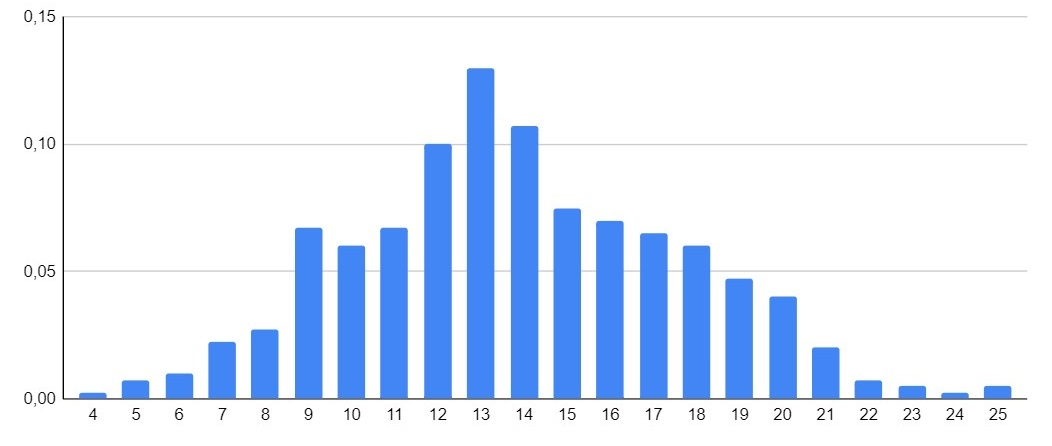
\includegraphics[scale=0.7]{Pics/hist1.jpg} \\
                    \textit{\textcolor[HTML]{000000}{Рис. 2. Гистограмма для t = 10 c}}
                \end{center}
            \end{minipage}
    
            \vspace*{0.6cm}

            \begin{minipage}[c]{\textwidth}
                \begin{center}
                    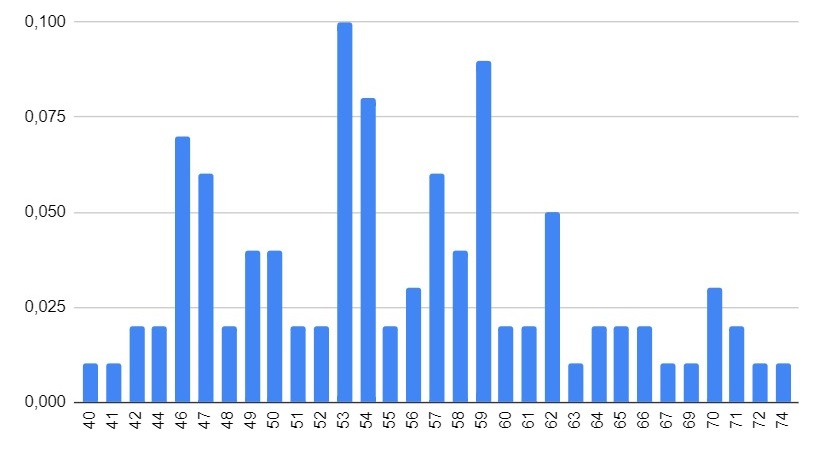
\includegraphics[scale=0.7]{Pics/hist2.jpg} \\
                    \textit{\textcolor[HTML]{000000}{Рис. 3. Гистограмма для t = 40 c}}
                \end{center}
            \end{minipage}

            \vspace*{0.6cm}
            \newpage
          {\large 3.3 Среднее число срабатываний счётчика за 10с. \\}

          $\overline{n_1} = \frac{1}{N_1} \sum_{i = 1}^{N_1} n_i = \frac{5539}{400} = 13.8475 $ \\

          {\large 3.4 Среднеквадратичная ошибка при t = 10с. \\}

            $\sigma_1 = \sqrt{\frac{1}{N_1} \sum_{i = 1}^{N_1} (n_i - \overline{n_1})^2} = \sqrt{\frac{5388}{400}} = 3.67$ \\
            Сравним $\sqrt{\overline{n_1}}$ и $\sigma_1$
            $\sqrt{\overline{n_1}} \approx 3.8 \approx 3.82 = \sigma_1$
            Получаем, что они равны. \\

          {\large 3.5 Доля случаев, когда отклонения от среднего значения $\leq \sigma_1 или \leq \sigma_2$ \\}

          \begin{center}
            \begin{tabular}{ |c|c|c|c| } \hline
            Ошибка & Число случаев & Доля случаев & Теоритическая оценка \\ \hline 
            $\pm 3.8$ & 246 & 61\% & 68\% \\ \hline 
            $\pm 7.6$ & 383 & 96\% & 95\% \\ \hline
            \end{tabular}
            \captionof{table}{Отклонения от среднего}
            \end{center} 
  

          {\large 3.6 Среднее число срабатываний счетчика за 40с \\}
          
          $\overline{n_2} = \frac{1}{N_2} \sum_{i = 1}^{N_2} n_i = \frac{5539}{100} = 55.39 $ \\

          {\large 3.7 Среднеквадратичная ошибка при t = 40с. \\}

          $\sigma_2 = \sqrt{\frac{1}{N_2} \sum_{i = 1}^{N_2} (n_i - \overline{n_2})^2} = \sqrt{\frac{4802}{100}} = 6.9$ \\
          Сравним $\sqrt{\overline{n_2}}$ и $\sigma_2$
          $\sqrt{\overline{n_2}} \approx 7.2 \approx 6.9 = \sigma_2$ \\
          
          {\large 3.8 Сравнение ошибок для t = 10c и t = 40c \\}
          $\overline{n_1} = 12.9; \sigma_1 = 3.7; \frac{\sigma_1}{\overline{n_1}} = 29\% $ \\
          $\overline{n_2} = 51.6; \sigma_2 = 6.9; \frac{\sigma_2}{\overline{n_2}} = 13\% $ \\
          
          {\large 3.9 Стандартная ошибка среднего значения (выборочного) $\overline{{n_1}}$ \\}
          $\sigma_{\overline{n_1}} = \frac{\sigma_1}{\sqrt{N_1}} \approx 0.18 $ \\
          Найдём относительную ошибку $\epsilon_{\overline{n_1}} = \frac{\sigma_{\overline{n_1}}}{\overline{n_1}} \approx 1.3 \%$ \\
          Такую относительную ошибку можно найти по формуле: \\
          $\epsilon_{\overline{n_1}} = \frac{1}{\sqrt{\overline{n_1} N_1}} \approx 1.4\%$ \\
            \underline{Окончательный результат:} $13.85 \pm 0.18$ 
            \vspace*{0.3cm}

          {\large 3.10 Стандартная ошибка среднего значения (выборочно) $\overline{{n_2}}$ \\}

          $\sigma_{\overline{n_2}} = \frac{\sigma_2}{\sqrt{N_2}} \approx 0.67 $ \\
          Найдём относительную ошибку $\epsilon_{\overline{n_2}} = \frac{\sigma_{\overline{n_2}}}{\overline{n_2}} \approx 1.3 \%$ \\
          Такую относительную ошибку можно найти по формуле: \\
          $\epsilon_{\overline{n_2}} = \frac{1}{\sqrt{\overline{n_2} N_2}} \approx 1.2\%$ \\
            \underline{Окончательный результат:} $55.4 \pm 0.7$ \\ 

          {\Large 4. Вывод: \\}
          Ознакомились с счётчиком Гейгера, применили методы обработки экспериментальных данных, изучили статистические закономерности, проверили на правильность формулы из теории вероятности.
        
\end{document}